\chapter{Experiment}
\label{chap:experiment}
In this chapter we discuss the application of our approach from Chapter~\ref{chap:approach} using an experiment. We describe how we setup and conduct our experiment in Section~\ref{sec:experiment_setup}. We describe the selected test subjects using general metrics in Section~\ref{sec:experiment_subjects}. Finally we display our experimental results in Section~\ref{sec:experiment_results}.


\section{Experimental Setup}
\label{sec:experiment_setup}
We run our approach on a machine that has 6 GB of \gls{ram} and an Intel Core i7-870 processor running at 2.93 GHz. We have configured Javalanche to run with no parallel task execution along with its coverage impact analysis. We avoid task parallelization as it avoids any unnecessary issues that can occur due to concurrent access to file resources that a test suite may use. The coverage impact analysis slows down Javalanche though it provides comprehensive data regarding the mutants.

For each test subject we import the project into Eclipse and run the project through a \emph{test} that Javalanche provides. This test indicates any unit test cases that cannot execute properly or fail within Javalanche. We have to remove these test cases as the mutation testing process requires a test suite with no errors. We collect all the results in a database so we can conduct several forms of evaluation.

Using the common classifier performance measures as described in Section~\ref{subsec:background_performance_measures} we can quantifier how well the classifier does at prediction. We perform 10-fold cross-validation as described in Section~\ref{sec:background_machine_learning}. We also observe the performance of the classifier on real predictions by training on a subset of the available data then predicting on the remaining subset. LIBSVM provides an \emph{easy script} that automatically scale the data and make parameter selection using a grid search~\cite{HCL03}. Parameter selection is critical aspect of machine learning algorithms, it can influence the classification accuracy greatly. We allow LIBSVM to automatically take care of this to best select the parameters based on the provided data. We allow LIBSVM to use 8 threads for computation tasks. We also utilize the \gls{rbf} kernel as it is the default and comes recommended by the authors~\cite{HCL03}.


\section{Experimental Subjects}
\label{sec:experiment_subjects}
Our selection criteria for the experimental subjects were the following:

\begin{itemize}
  \item An open source Java software system.
  \item Contains a test suite or set of test cases.
  \item Is over 5K total \gls{sloc}.
\end{itemize}

We only wanted software system that have a minimum of 5K total \gls{sloc} to ensure that the our approach would gather a decent amount of data. Open source projects are relatively easy to find and are freely available to analyze. The only firm requirement we desired was the need for a test suite or set of test cases, due to fundamental needs of mutation testing.

\begin{landscape}
  \begin{table}[t]
    \centering
    \rowcolors{2}{gray!30}{gray!20}
    \begin{tabular}{|l|>{\raggedleft\arraybackslash}p{1.9cm}|>{\raggedleft\arraybackslash}p{1.9cm}|>{\raggedleft\arraybackslash}p{1.9cm}|>{\raggedleft\arraybackslash}p{1.9cm}|>{\raggedleft\arraybackslash}p{1.9cm}|>{\raggedleft\arraybackslash}p{1.9cm}|>{\raggedleft\arraybackslash}p{1.9cm}|}
      \hline
      \rowcolor[RGB]{169,196,223}
      \textbf{Program} & \textbf{Source SLOC} & \textbf{Source Classes} & \textbf{Source Methods} & \textbf{Test SLOC} & \textbf{Test Classes} & \textbf{Test Methods} & \textbf{Test Cases} \\
      \hline logback-core (1.0.3)~\cite{logback} & 12118 & 249 & 1270 & 8377 & 174 & 688 & 286 \\
      \hline barbecue (1.5-beta1)~\cite{barbecue} & 4790 & 58 & 299 & 2910 & 38 & 416 & 225 \\
      \hline jgap (3.6.1)~\cite{jgap} & 28975 & 415 & 3017 & 19694 & 180 & 1633 & 1355 \\
      \hline commons-lang (3.1)~\cite{commons-lang} & 19499 & 149 & 1196 & 33332 & 242 & 2408 & 2050 \\
      \hline joda-time (2.0)~\cite{joda-time} & 27139 & 227 & 3635 & 51388 & 221 & 4755 & 3866 \\
      \hline openfast (1.1.0)~\cite{openfast} & 11646 & 265 & 1447 & 5587 & 115 & 421 & 322 \\
      \hline jsoup (1.6.2)~\cite{jsoup} & 10949 & 198 & 954 & 2883 & 25 & 335 & 319 \\
      \hline joda-primitives (1.0)~\cite{joda-primitives} & 11157 & 128 & 1868 & 6989 & 49 & 746 & 1810 \\
      \hline \textbf{ALL} & \textbf{126273} & \textbf{1689} & \textbf{13686} & \textbf{131160} & \textbf{1044} & \textbf{11402} & \textbf{10233} \\
      \hline
    \end{tabular}
    \caption{The set of experimental subjects along with source and test metrics.}
    \vspace{2mm}
    \hrule
    \label{tab:experimental_subjects}
  \end{table}
\end{landscape}

Following the criteria outlined we selected the following 8 open source Java projects shown in Table~\ref{tab:experimental_subjects}. We provide a brief description of each project:

\begin{itemize}
  \item \textbf{logback-core}: \emph{``Logback is intended as a successor to the popular log4j project, picking up where log4j leaves off. The logback-core module lays the groundwork for the other two modules.''}~\cite{logback}
  \item \textbf{barbecue}: \emph{``Barbecue is an open-source, Java library that provides the means to create barcodes for printing and display in Java applications.''}~\cite{barbecue}
  \item \textbf{jgap}: \emph{``JGAP is a Genetic Algorithms and Genetic Programming component provided as a Java framework.''}~\cite{jgap}
  \item \textbf{commons-lang}: \emph{``The standard Java libraries fail to provide enough methods for manipulation of its core classes. Apache Commons Lang provides these extra methods.''}\cite{commons-lang}
  \item \textbf{joda-time}: \emph{``Joda-Time provides a quality replacement for the Java date and time classes. The design allows for multiple calendar systems, while still providing a simple API.''}~\cite{joda-time}
  \item \textbf{openfast}: \emph{``OpenFAST is a 100\% Java implementation of the FAST Protocol (FIX Adapted for STreaming). The FAST protocol is used to optimize communications in the electronic exchange of financial data.''}~\cite{openfast}
  \item \textbf{jsoup}: \emph{``jsoup is a Java library for working with real-world HTML. It provides a very convenient API for extracting and manipulating data, using the best of DOM, CSS, and jquery-like methods.''}~\cite{jsoup}
  \item \textbf{joda-primitives}: \emph{``Joda Primitives provides collections and utilities to bridge the gap between objects and primitive types in Java.''}~\cite{joda-primitives}
\end{itemize}

We use these experimental subjects in combination while collecting results. We consider an \emph{all} set which contains the data from all individual subjects, this allows us to observe the results using an amalgamation of subjects. We also consider subsets of the \emph{all} set by omitting a different subject for each subset (i.e., \emph{all\_but\_<subject>}), this allows us to perform predictions on a completely unknown subject using that data of the 7 other subjects.


\section{Experimental Results}
\label{sec:experiment_results}
Our results are broken up into separate sections:

\begin{itemize}
  \item \textbf{Mutation Score Distribution (Section~\ref{subsec:experiment_mutation_score_distribution})}: We discuss the results of the mutation score collection of the source code units. This section outlines the raw data and observations regarding the distribution of mutation scores. In particular we identify a suitable category abstraction for the mutation scores before moving forward to training and prediction using a \gls{svm}.
  \item \textbf{Cross Validation (Section~\ref{subsec:experiment_cross_validation})}: We discuss the cross-validation accuracy of our data sets. We present the cross-validation accuracy results with respect to the feature sets outlined in Table~\ref{tab:metrics}.
  \item \textbf{Feature Selection (Section~\ref{subsec:experiment_feature_selection})}: We discuss ways to optimize our feature set by reducing redundant and detrimental attributes. The results of the feature selection process are presented using the \emph{all} project.
  \item \textbf{Prediction (Section~\ref{subsec:experiment_prediction})}: We discuss our approach and results on predicting unknown subjects using the collected data from our subjects.
  \item \textbf{Optimization \& Generalization (Section~\ref{subsec:experiment_optimization_generalization})}: We discuss the benefits of finding a generalizable set of parameters that fit our prediction purposes. We then re-evaluate the cross-validation and prediction accuracy using the optimized subset of features (from Section~\ref{subsec:experiment_feature_selection}) with generalized parameters.
\end{itemize}


\subsection{Mutation Score Distribution}
\label{subsec:experiment_mutation_score_distribution}
\begin{landscape}
  \begin{table}[]
    \centering
    \rowcolors{1}{gray!30}{gray!20}
    \begin{threeparttable}
      \begin{tabular}{|l|>{\raggedleft}p{2.5cm}|>{\raggedleft}p{2.5cm}|>{\raggedleft}p{2.5cm}|>{\raggedleft}p{2.5cm}|>{\raggedleft}p{2.5cm}|>{\raggedleft\arraybackslash}p{2.5cm}|}
        \rowcolor[RGB]{169,196,223}
        \hline & \textbf{Mutants Generated} & \textbf{Mutants Covered} & \textbf{Coverage Percent} & \textbf{Mutants Killed} & \textbf{Mutation Score\tnote{a}} & \textbf{Time Taken (\emph{hh:mm:ss})} \\
        \hline \cellcolor[RGB]{169,196,223} \textbf{logback-core} & 10682 & 7350 & 0.6881 & 5400 & 0.7347 & 01:49:10 \\
        \hline \cellcolor[RGB]{169,196,223} \textbf{barbecue} & 27324 & 4339 & 0.1588 & 2727 & 0.6285 & 00:49:51 \\
        \hline \cellcolor[RGB]{169,196,223} \textbf{jgap} & 31929 & 17903 & 0.5607 & 13328 & 0.7445 & 07:04:44 \\
        \hline \cellcolor[RGB]{169,196,223} \textbf{commons-lang} & 45141 & 41761 & 0.9251 & 33772 & 0.8087 & 15:51:59 \\
        \hline \cellcolor[RGB]{169,196,223} \textbf{joda-time} & 70594 & 58595 & 0.8300 & 48545 & 0.8285 & 31:55:50 \\
        \hline \cellcolor[RGB]{169,196,223} \textbf{openfast} & 14910 & 8371 & 0.5614 & 6869 & 0.8206 & 01:34:38 \\
        \hline \cellcolor[RGB]{169,196,223} \textbf{jsoup} & 14165 & 10540 & 0.7441 & 8430 & 0.7998 & 03:55:56 \\
        \hline \cellcolor[RGB]{169,196,223} \textbf{joda-primitives} & 22269 & 17334 & 0.7784 & 13499 & 0.7788 & 01:24:33 \\
        \hline \cellcolor[RGB]{169,196,223} \textbf{ALL} & \textbf{237014} & \textbf{166193} & \textbf{0.7012} & \textbf{132570} & \textbf{0.7786} & \textbf{64:26:41} \\
        \hline
      \end{tabular}
      \begin{tablenotes}
        \item[a] Mutation score is calculated using the covered and killed mutants.
      \end{tablenotes}
    \end{threeparttable}
    \caption{Mutation testing results of the experimental subjects from table~\ref{tab:experimental_subjects}.}
    \vspace{2mm}
    \hrule
    \label{tab:experiments_mutation_results}
  \end{table}

  \begin{table}[ht!]
    \centering
    \rowcolors{1}{gray!30}{gray!20}
    \begin{threeparttable}
      \begin{tabular}{|l|r|r|}
        \rowcolor[RGB]{169,196,223}
        \hline & \textbf{Class-Level} & \textbf{Method-Level} \\
        \hline \cellcolor[RGB]{169,196,223} \textbf{logback-core} & 115 & 447 \\
        \hline \cellcolor[RGB]{169,196,223} \textbf{barbecue} & 31 & 143 \\
        \hline \cellcolor[RGB]{169,196,223} \textbf{jgap} & 124 & 655 \\
        \hline \cellcolor[RGB]{169,196,223} \textbf{commons-lang} & 124 & 789 \\
        \hline \cellcolor[RGB]{169,196,223} \textbf{joda-time} & 194 & 2019 \\
        \hline \cellcolor[RGB]{169,196,223} \textbf{openfast} & 120 & 401 \\
        \hline \cellcolor[RGB]{169,196,223} \textbf{jsoup} & 83 & 381 \\
        \hline \cellcolor[RGB]{169,196,223} \textbf{joda-primitives} & 73 & 675 \\
        \hline \cellcolor[RGB]{169,196,223} \textbf{ALL} & \textbf{864} & \textbf{5510} \\
        \hline
      \end{tabular}
    \end{threeparttable}
    \caption{The usable number of source code unit data points gathered from the experimental subjects in table~\ref{tab:experimental_subjects}.}
    \vspace{2mm}
    \hrule
    \label{tab:experiments_collected_data}
  \end{table}
\end{landscape}

As described in Chapter~\ref{chap:approach} our approach uses mutation testing to acquire the necessary mutation score data used for the category of the source code units. Table~\ref{tab:experiments_mutation_results} shows the results of running Javalanche on our experimental subjects. In all of our subjects mutation testing produced a large number of mutants that were evaluated, taking just over 64 hours for the entire mutation testing process. As described in Section~\ref{subsec:background_mutation_tools} Javalanche utilizes \emph{coverage} (i.e., basic block coverage) for test selection, which limits the number of mutants to evaluate to a subset of covered mutants. In most cases Javalanche was able to kill a reasonable percentage of the covered mutants with a mutation score of 0.7786 using all projects cumulatively. From the table we can see that the mutation scores of the individual projects are mostly above 0.7 which is a good indication that the test suites for covered source code units are reasonably effective. The coverage percent overall is 0.7012 which indicates that the test suites of the projects did not cover about 30\% of the generated mutants. Realistically mutation test works off of the entire project's source code, for our purpose only covered mutants were used to calculate the mutation score. The corrective action for non-covered mutants (i.e., mutants not covered by test suite using basic block coverage) is to add new test cases that provide coverage over the mutant's location.

\begin{figure}[ht!]
  \centering
  \begin{tikzpicture}
  \begin{axis}[
      bar width=1,
      ymajorgrids=true,
      xlabel=Mutation Score (\%),
      ylabel=\# of Classes,
      width=\linewidth,
      height=9.0cm]
      \addplot[ybar,fill=black] file {plots/all/evaluation_projects_class_distribution.txt};
  \end{axis}
  \end{tikzpicture}
  \caption{Mutation score distribution of classes from all 8 subjects from Table~\ref{tab:experimental_subjects} that can be used for training.}
  \vspace{2mm}
  \hrule
  \label{fig:mutation_distributions_class_all}
\end{figure}

\begin{figure}[ht!]
  \centering
  \begin{tikzpicture}
  \begin{axis}[
      bar width=1,
      ymajorgrids=true,
      xlabel=Mutation Score (\%),
      ylabel=\# of Methods,
      width=\linewidth,
      height=9.0cm]
      \addplot[ybar,fill=black] file {plots/all/evaluation_projects_method_distribution.txt};
  \end{axis}
  \end{tikzpicture}
  \caption{Mutation score distribution of methods from all 8 subjects from Table~\ref{tab:experimental_subjects} that can be used for training.}
  \vspace{2mm}
  \hrule
  \label{fig:mutation_distributions_method_all}
\end{figure}

\begin{figure}[ht!]
  \centering
  \begin{tikzpicture}
  \begin{axis}[
      xtick={0, 25, 50, 75, 100, 125, 150, 175, 200},
      xticklabels={0, 25, 50, 75, 100, 125, 150, 175, 200>=},
      bar width=1,
      ymajorgrids=true,
      xlabel=\# of Covered Mutants,
      ylabel=\# of Classes,
      width=\linewidth,
      height=9.0cm]
      \addplot[ybar,fill=black] file {plots/all/covered_mutants_class_distribution.txt};
  \end{axis}
  \end{tikzpicture}
  \caption{Covered mutant distribution of classes from all 8 subjects from Table~\ref{tab:experimental_subjects} that can be used for training.}
  \vspace{1mm}
  \footnotesize{\emph{Figure~\ref{fig:covered_mutant_distributions_class_all} only presents a subset of the full distribution, with the excluded values added on the last visible value. The max number of covered mutants found was 6507, which corresponds to the following class \texttt{org.joda.time.format.ISODateTimeFormat} from the \texttt{joda-time} project.}}
  \vspace{2mm}
  \hrule
  \label{fig:covered_mutant_distributions_class_all}
\end{figure}

\begin{figure}[ht!]
  \centering
  \begin{tikzpicture}
  \begin{axis}[
      xtick={0, 25, 50, 75, 100, 125, 150, 175, 200},
      xticklabels={0, 25, 50, 75, 100, 125, 150, 175, 200>=},
      bar width=1,
      ymajorgrids=true,
      xlabel=\# of Covered Mutants,
      ylabel=\# of Methods,
      width=\linewidth,
      height=9.0cm]
      \addplot[ybar,fill=black] file {plots/all/covered_mutants_method_distribution.txt};
  \end{axis}
  \end{tikzpicture}
  \caption{Covered mutant distribution of methods from all 8 subjects from Table~\ref{tab:experimental_subjects} that can be used for training.}
  \vspace{1mm}
  \footnotesize{\emph{Figure~\ref{fig:covered_mutant_distributions_method_all} only presents a subset of the full distribution, with the excluded values added on the last visible value. The max number of covered mutants found was 587, which corresponds to the following method \texttt{org.joda.time.format.PeriodFormatterBuilder\$FieldFormatter.parseInto} from the \texttt{joda-time} project. There were also 51 methods that had 117 covered mutants, of these 48 all fall within the \texttt{ISODateTimeFormat} class within the \texttt{joda-time} project.}}
  \vspace{2mm}
  \hrule
  \label{fig:covered_mutant_distributions_method_all}
\end{figure}

Source code and test code metrics were collected as described in Chapter~\ref{chap:approach} which represents the set of feature data that make up the vectors of our \gls{svm}. Our approach can only make predictions using the synthesis of both mutation score data (i.e., category data) and source and test suite metrics (i.e., feature data) of source code units. If any piece of data is missing then we cannot use that source code unit for training and prediction purposes. Using our approach we collected data for 864 class-level and 5510 method-level source code units shown in Table~\ref{tab:experiments_collected_data}. The collected data items is lower then the total available methods and classes, this is because: we ignore abstract, anonymous and overloaded source code units, as well as any source units with missing data (i.e., no tests cases). We present the distribution of the all the collected data points for both class-level and method-level source code units with respect to mutation score in Figure~\ref{fig:mutation_distributions_class_all}~\&~\ref{fig:mutation_distributions_method_all}. The mutation score distributions for each individual project are found in Appendix~\ref{app:mutation_score_distributions}. The mutation distribution of the both class-level and method-level source code units are both negatively skewed which confirms our earlier observation that the test suite for the collected source code units are reasonably strong at detecting faults. The 0\%, 50\% and 100\% values for mutation score contain significantly more data points then their surroundings, in particular the 100\% is ranges 2--9 times more dense then other areas respectively. We speculate this occurs because a large number of source code units probably have small number of covered mutants (i.e., easier to kill all, evenly kill half, kill none). Analysis of the covered mutant distribution for class-level source code units (as seen in Figure~\ref{fig:covered_mutant_distributions_method_all}) shows a slightly denser grouping for low covered mutants. The covered mutant distribution for method-level source code units supports our speculation, the distribution is positively skewed. With respect to the percentile of the class-level distribution of covered mutants a \sfrac{1}{4} of the classes have less then 16 covered mutants. The method-level results show that \sfrac{1}{4} of the methods have less then 2 covered mutants, furthermore \sfrac{1}{2} of the method have less then 6 covered mutants. With distributions like this we can assure that our speculation of many low covered mutant that can contribute to the high 0\%, 50\% and 100\% values for mutation score.

Earlier in Section~\ref{subsec:approach_create_libsvm_file} we mentioned that our approached would create \emph{.libsvm} files using the acquire data. The category data required for the files that the \gls{svm} utilizes is based on the mutation score of source code units. To avoid predicting the exact mutation score which is a set of real numbers, we instead use an abstracted set of categories (i.e., ranges of mutation scores). We were unsure on how to properly select the ranges to use for our categories. We decided to base our categories on the distribution of mutation scores from Figure~\ref{fig:covered_mutant_distributions_class_all}~\&~\ref{fig:covered_mutant_distributions_method_all}. We found that the class-level distribution has a 25$^{th}$, 50$^{th}$ and 75$^{th}$ percentile of 0.72, 0.81, 0.89 respectively, and for same percentiles of the method-level distribution are 0.75, 0.87, 0.99. Using these values we decided to use the following as our general case for categories:

\begin{itemize}
  \item \textbf{LOW} = [0.00--0.70)
  \item \textbf{MEDIUM} = [0.70--0.90)
  \item \textbf{HIGH} = [0.90--1.00]
\end{itemize}

The rational behind the categories is separate the lower and upper percentiles in to the LOW and HIGH category, with the remaining into the MEDIUM category. We believe that these values will provide a sufficient level of information over the mutation testing coverage of the source code units.


\subsection{Cross Validation}
\label{subsec:experiment_cross_validation}
\begin{table}[ht!]
  \centering
  \rowcolors{2}{gray!30}{gray!20}
  \begin{tabular}{|l|>{\raggedleft\arraybackslash}p{3cm}|>{\raggedleft\arraybackslash}p{3cm}|>{\raggedleft\arraybackslash}p{3cm}|}
    \hline
    \rowcolor[RGB]{169,196,223}
    \textbf{Category} & \textbf{Mutation Score Range} & \textbf{Class-Level Units} & \textbf{Method-Level Units} \\
    \hline LOW & [0.00--0.70) & 191 & 1104 \\
    \hline MEDIUM & [0.70--0.90) & 459 & 1782 \\
    \hline HIGH & [0.90--1.00] & 214 & 2624 \\
    \hline
  \end{tabular}
  \caption{The available number of source code units that fall within the determined ranges of mutation scores.}
  \vspace{2mm}
  \label{tab:available_data}
\end{table}

Using the determined classification categories from the previous section we have imbalanced training data in each category for class- and method-level source code units as shown in Table~\ref{tab:available_data}. Imbalanced data can be problematic for training and predicting using machine learning techniques. With imbalanced data a classifier will heavily classify towards the majority category~\cite{BOSB10}. Barandela et al. indicate that there are three strategies to reduce the problem of imbalanced training data: Over-sample, under-sample, or internally bias the classification process~\cite{BVSF04}. It was shown that simple random under-sampling can be an effective solution (though not always the best) to this problem~\cite{Jap00,AKJ04}. As Akbani et al. mentioned \emph{``\ldots we are throwing away valid instances, which contain valuable information''}, therefore we might be limiting the ability to generalize to new unknown data~\cite{AKJ04}. The alternative is to perform over-sampling, as Batista et al. mention \emph{``\ldots random over-sampling can increase the likelihood of occurring overfitting, since it makes exact copies of the minority class examples''}~\cite{BPM04}. We decided to utilize random under-sampling as it provides a simple approach to dealing with imbalanced data. Furthermore the imbalanced data we have is not extremely severe with a ratio around 2:5, thus we believe we are not losing that much information by under-sampling our training data.

\begin{figure}[ht!]
  \centering
  \begin{adjustbox}{max size={.95\textwidth}{.95\textheight}}
    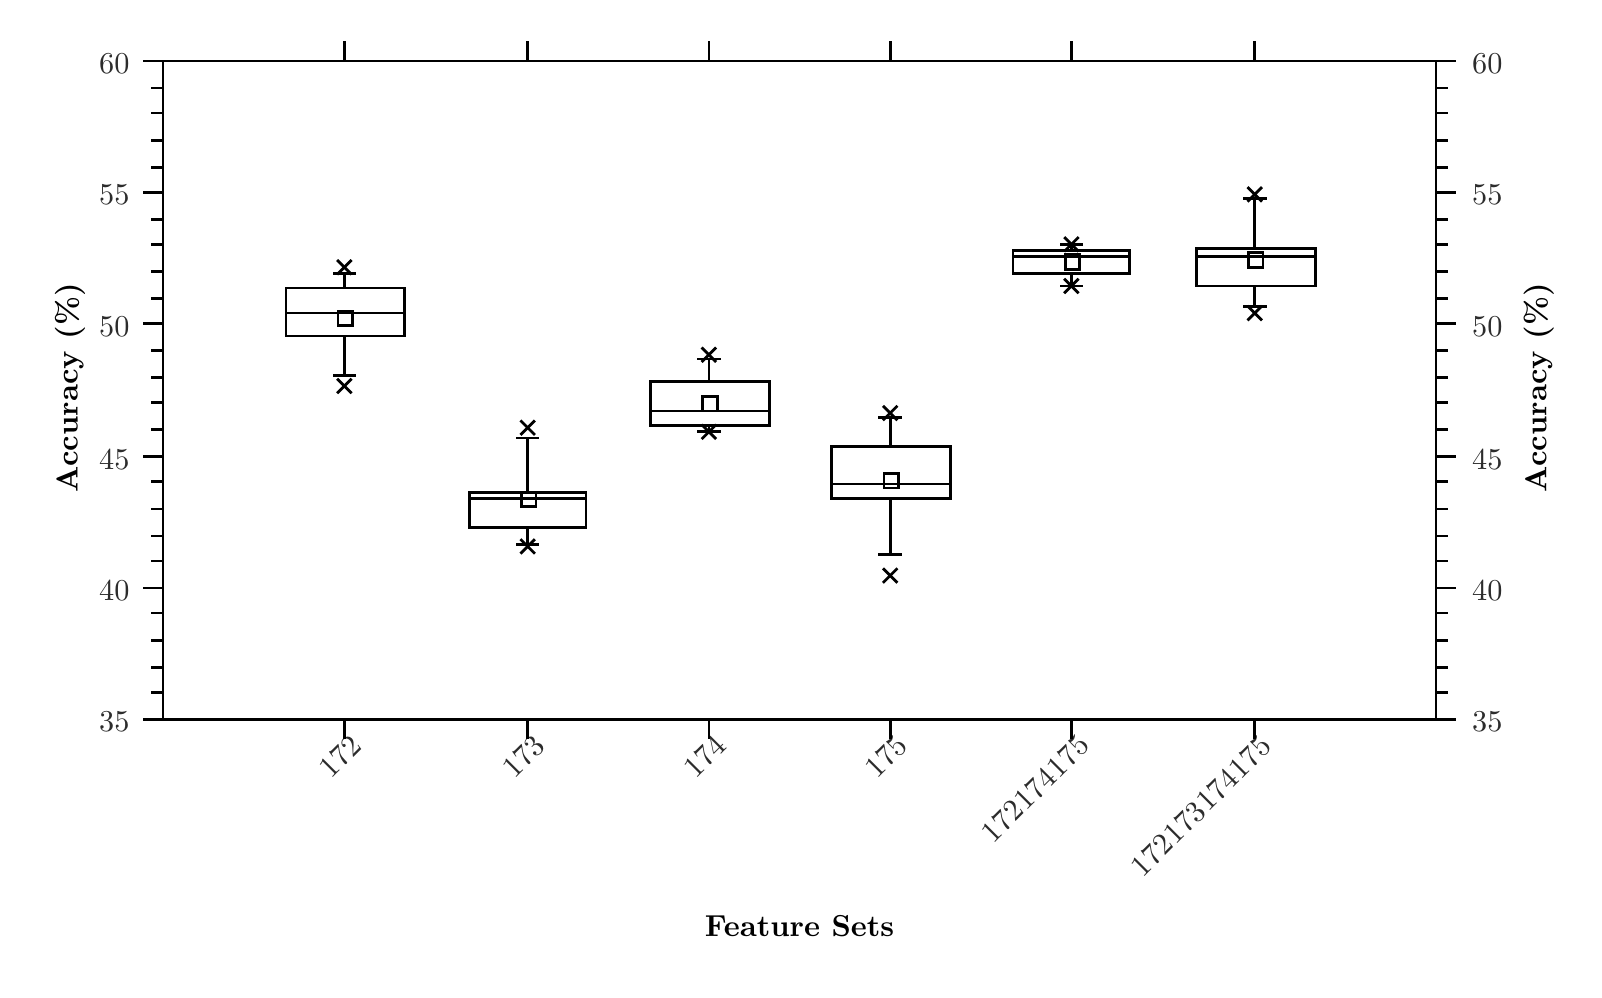
\begin{tikzpicture}{0pt}{0pt}{742pt}{452pt}
	\clip(0pt,452pt) -- (558.587pt,452pt) -- (558.587pt,111.729pt) -- (0pt,111.729pt) -- (0pt,452pt);
\begin{scope}
	\clip(48.9328pt,439.955pt) -- (508.901pt,439.955pt) -- (508.901pt,202.066pt) -- (48.9328pt,202.066pt) -- (48.9328pt,439.955pt);
	\color[rgb]{0,0,0}
	\draw[line width=1pt, line join=miter, line cap=rect](93.3487pt,357.898pt) -- (136.259pt,357.898pt) -- (136.259pt,340.584pt) -- (93.3487pt,340.584pt) -- (93.3487pt,357.898pt);
	\color[rgb]{0,0,0}
	\draw[line width=1pt, line join=miter, line cap=rect](110.663pt,326.28pt) -- (118.192pt,326.28pt);
	\draw[line width=1pt, line join=miter, line cap=rect](110.663pt,363.168pt) -- (118.192pt,363.168pt);
	\draw[line width=1pt, line join=miter, line cap=rect](114.427pt,363.168pt) -- (114.427pt,357.898pt);
	\draw[line width=1pt, line join=miter, line cap=rect](114.427pt,326.28pt) -- (114.427pt,340.584pt);
	\draw[line width=1pt, line join=miter, line cap=rect](93.3487pt,348.865pt) -- (135.506pt,348.865pt);
	\draw[line width=1pt, line join=miter, line cap=rect](112.169pt,324.775pt) -- (116.686pt,320.258pt);
	\draw[line width=1pt, line join=miter, line cap=rect](112.169pt,320.258pt) -- (116.686pt,324.775pt);
	\draw[line width=1pt, line join=miter, line cap=rect](112.169pt,367.685pt) -- (116.686pt,363.168pt);
	\draw[line width=1pt, line join=miter, line cap=rect](112.169pt,363.168pt) -- (116.686pt,367.685pt);
	\draw[line width=1pt, line join=miter, line cap=rect](112.169pt,349.618pt) -- (117.439pt,349.618pt) -- (117.439pt,344.348pt) -- (112.169pt,344.348pt) -- (112.169pt,349.618pt);
	\draw[line width=1pt, line join=miter, line cap=rect](159.596pt,284.123pt) -- (201.754pt,284.123pt) -- (201.754pt,271.325pt) -- (159.596pt,271.325pt) -- (159.596pt,284.123pt);
	\draw[line width=1pt, line join=miter, line cap=rect](176.911pt,265.303pt) -- (184.439pt,265.303pt);
	\draw[line width=1pt, line join=miter, line cap=rect](176.911pt,303.696pt) -- (184.439pt,303.696pt);
	\draw[line width=1pt, line join=miter, line cap=rect](180.675pt,303.696pt) -- (180.675pt,284.123pt);
	\draw[line width=1pt, line join=miter, line cap=rect](180.675pt,265.303pt) -- (180.675pt,271.325pt);
	\draw[line width=1pt, line join=miter, line cap=rect](159.596pt,281.864pt) -- (201.754pt,281.864pt);
	\draw[line width=1pt, line join=miter, line cap=rect](178.417pt,266.808pt) -- (182.933pt,262.291pt);
	\draw[line width=1pt, line join=miter, line cap=rect](178.417pt,262.291pt) -- (182.933pt,266.808pt);
	\draw[line width=1pt, line join=miter, line cap=rect](178.417pt,309.718pt) -- (182.933pt,305.202pt);
	\draw[line width=1pt, line join=miter, line cap=rect](178.417pt,305.202pt) -- (182.933pt,309.718pt);
	\draw[line width=1pt, line join=miter, line cap=rect](178.417pt,284.123pt) -- (183.686pt,284.123pt) -- (183.686pt,278.853pt) -- (178.417pt,278.853pt) -- (178.417pt,284.123pt);
	\draw[line width=1pt, line join=miter, line cap=rect](225.091pt,324.022pt) -- (268.001pt,324.022pt) -- (268.001pt,308.213pt) -- (225.091pt,308.213pt) -- (225.091pt,324.022pt);
	\draw[line width=1pt, line join=miter, line cap=rect](242.406pt,305.954pt) -- (249.934pt,305.954pt);
	\draw[line width=1pt, line join=miter, line cap=rect](242.406pt,332.303pt) -- (249.934pt,332.303pt);
	\draw[line width=1pt, line join=miter, line cap=rect](246.17pt,332.303pt) -- (246.17pt,324.022pt);
	\draw[line width=1pt, line join=miter, line cap=rect](246.17pt,305.954pt) -- (246.17pt,308.213pt);
	\draw[line width=1pt, line join=miter, line cap=rect](225.091pt,313.482pt) -- (267.248pt,313.482pt);
	\draw[line width=1pt, line join=miter, line cap=rect](243.911pt,308.213pt) -- (248.428pt,303.696pt);
	\draw[line width=1pt, line join=miter, line cap=rect](243.911pt,303.696pt) -- (248.428pt,308.213pt);
	\draw[line width=1pt, line join=miter, line cap=rect](243.911pt,336.067pt) -- (248.428pt,331.55pt);
	\draw[line width=1pt, line join=miter, line cap=rect](243.911pt,331.55pt) -- (248.428pt,336.067pt);
	\draw[line width=1pt, line join=miter, line cap=rect](243.911pt,318.752pt) -- (249.181pt,318.752pt) -- (249.181pt,313.482pt) -- (243.911pt,313.482pt) -- (243.911pt,318.752pt);
	\draw[line width=1pt, line join=miter, line cap=rect](290.586pt,300.685pt) -- (333.496pt,300.685pt) -- (333.496pt,281.864pt) -- (290.586pt,281.864pt) -- (290.586pt,300.685pt);
	\draw[line width=1pt, line join=miter, line cap=rect](307.9pt,261.538pt) -- (315.428pt,261.538pt);
	\draw[line width=1pt, line join=miter, line cap=rect](307.9pt,311.224pt) -- (315.428pt,311.224pt);
	\draw[line width=1pt, line join=miter, line cap=rect](311.664pt,311.224pt) -- (311.664pt,300.685pt);
	\draw[line width=1pt, line join=miter, line cap=rect](311.664pt,261.538pt) -- (311.664pt,281.864pt);
	\draw[line width=1pt, line join=miter, line cap=rect](290.586pt,287.134pt) -- (332.743pt,287.134pt);
	\draw[line width=1pt, line join=miter, line cap=rect](309.406pt,256.269pt) -- (313.923pt,251.752pt);
	\draw[line width=1pt, line join=miter, line cap=rect](309.406pt,251.752pt) -- (313.923pt,256.269pt);
	\draw[line width=1pt, line join=miter, line cap=rect](309.406pt,314.988pt) -- (313.923pt,310.471pt);
	\draw[line width=1pt, line join=miter, line cap=rect](309.406pt,310.471pt) -- (313.923pt,314.988pt);
	\draw[line width=1pt, line join=miter, line cap=rect](309.406pt,290.898pt) -- (314.676pt,290.898pt) -- (314.676pt,285.628pt) -- (309.406pt,285.628pt) -- (309.406pt,290.898pt);
	\draw[line width=1pt, line join=miter, line cap=rect](356.08pt,371.449pt) -- (398.238pt,371.449pt) -- (398.238pt,363.168pt) -- (356.08pt,363.168pt) -- (356.08pt,371.449pt);
	\draw[line width=1pt, line join=miter, line cap=rect](373.395pt,358.651pt) -- (380.923pt,358.651pt);
	\draw[line width=1pt, line join=miter, line cap=rect](373.395pt,373.707pt) -- (380.923pt,373.707pt);
	\draw[line width=1pt, line join=miter, line cap=rect](377.159pt,373.707pt) -- (377.159pt,371.449pt);
	\draw[line width=1pt, line join=miter, line cap=rect](377.159pt,358.651pt) -- (377.159pt,363.168pt);
	\draw[line width=1pt, line join=miter, line cap=rect](356.08pt,369.191pt) -- (398.238pt,369.191pt);
	\draw[line width=1pt, line join=miter, line cap=rect](374.901pt,360.91pt) -- (379.418pt,356.393pt);
	\draw[line width=1pt, line join=miter, line cap=rect](374.901pt,356.393pt) -- (379.418pt,360.91pt);
	\draw[line width=1pt, line join=miter, line cap=rect](374.901pt,375.966pt) -- (379.418pt,371.449pt);
	\draw[line width=1pt, line join=miter, line cap=rect](374.901pt,371.449pt) -- (379.418pt,375.966pt);
	\draw[line width=1pt, line join=miter, line cap=rect](374.901pt,369.943pt) -- (380.17pt,369.943pt) -- (380.17pt,364.674pt) -- (374.901pt,364.674pt) -- (374.901pt,369.943pt);
	\draw[line width=1pt, line join=miter, line cap=rect](422.328pt,372.202pt) -- (465.238pt,372.202pt) -- (465.238pt,358.651pt) -- (422.328pt,358.651pt) -- (422.328pt,372.202pt);
	\draw[line width=1pt, line join=miter, line cap=rect](439.642pt,351.123pt) -- (447.171pt,351.123pt);
	\draw[line width=1pt, line join=miter, line cap=rect](439.642pt,390.269pt) -- (447.171pt,390.269pt);
	\draw[line width=1pt, line join=miter, line cap=rect](443.407pt,390.269pt) -- (443.407pt,372.202pt);
	\draw[line width=1pt, line join=miter, line cap=rect](443.407pt,351.123pt) -- (443.407pt,358.651pt);
	\draw[line width=1pt, line join=miter, line cap=rect](422.328pt,369.191pt) -- (464.485pt,369.191pt);
	\draw[line width=1pt, line join=miter, line cap=rect](441.148pt,351.123pt) -- (445.665pt,346.606pt);
	\draw[line width=1pt, line join=miter, line cap=rect](441.148pt,346.606pt) -- (445.665pt,351.123pt);
	\draw[line width=1pt, line join=miter, line cap=rect](441.148pt,394.033pt) -- (445.665pt,389.517pt);
	\draw[line width=1pt, line join=miter, line cap=rect](441.148pt,389.517pt) -- (445.665pt,394.033pt);
	\draw[line width=1pt, line join=miter, line cap=rect](441.148pt,370.696pt) -- (446.418pt,370.696pt) -- (446.418pt,365.427pt) -- (441.148pt,365.427pt) -- (441.148pt,370.696pt);
\end{scope}
\begin{scope}
	\color[rgb]{0,0,0}
	\pgftext[center, base, at={\pgfpoint{18.0675pt}{321.763pt}},rotate=90]{\fontsize{11}{0}\selectfont{\textbf{Accuracy (\%)}}}
	\color[rgb]{0.172549,0.172549,0.172549}
	\pgftext[center, base, at={\pgfpoint{31.3358pt}{197.549pt}}]{\fontsize{11}{0}\selectfont{35}}
	\pgftext[center, base, at={\pgfpoint{31.3358pt}{244.977pt}}]{\fontsize{11}{0}\selectfont{40}}
	\pgftext[center, base, at={\pgfpoint{31.3358pt}{292.404pt}}]{\fontsize{11}{0}\selectfont{45}}
	\pgftext[center, base, at={\pgfpoint{31.3358pt}{340.584pt}}]{\fontsize{11}{0}\selectfont{50}}
	\pgftext[center, base, at={\pgfpoint{31.3358pt}{388.011pt}}]{\fontsize{11}{0}\selectfont{55}}
	\pgftext[center, base, at={\pgfpoint{31.3358pt}{435.438pt}}]{\fontsize{11}{0}\selectfont{60}}
	\color[rgb]{0,0,0}
	\draw[line width=1pt, line join=bevel, line cap=rect](48.9328pt,211.853pt) -- (45.1688pt,211.853pt);
	\draw[line width=1pt, line join=bevel, line cap=rect](48.9328pt,220.887pt) -- (45.1688pt,220.887pt);
	\draw[line width=1pt, line join=bevel, line cap=rect](48.9328pt,230.673pt) -- (45.1688pt,230.673pt);
	\draw[line width=1pt, line join=bevel, line cap=rect](48.9328pt,240.46pt) -- (45.1688pt,240.46pt);
	\draw[line width=1pt, line join=bevel, line cap=rect](48.9328pt,259.28pt) -- (45.1688pt,259.28pt);
	\draw[line width=1pt, line join=bevel, line cap=rect](48.9328pt,268.314pt) -- (45.1688pt,268.314pt);
	\draw[line width=1pt, line join=bevel, line cap=rect](48.9328pt,278.1pt) -- (45.1688pt,278.1pt);
	\draw[line width=1pt, line join=bevel, line cap=rect](48.9328pt,287.887pt) -- (45.1688pt,287.887pt);
	\draw[line width=1pt, line join=bevel, line cap=rect](48.9328pt,306.707pt) -- (45.1688pt,306.707pt);
	\draw[line width=1pt, line join=bevel, line cap=rect](48.9328pt,316.494pt) -- (45.1688pt,316.494pt);
	\draw[line width=1pt, line join=bevel, line cap=rect](48.9328pt,325.528pt) -- (45.1688pt,325.528pt);
	\draw[line width=1pt, line join=bevel, line cap=rect](48.9328pt,335.314pt) -- (45.1688pt,335.314pt);
	\draw[line width=1pt, line join=bevel, line cap=rect](48.9328pt,354.134pt) -- (45.1688pt,354.134pt);
	\draw[line width=1pt, line join=bevel, line cap=rect](48.9328pt,363.921pt) -- (45.1688pt,363.921pt);
	\draw[line width=1pt, line join=bevel, line cap=rect](48.9328pt,373.707pt) -- (45.1688pt,373.707pt);
	\draw[line width=1pt, line join=bevel, line cap=rect](48.9328pt,382.741pt) -- (45.1688pt,382.741pt);
	\draw[line width=1pt, line join=bevel, line cap=rect](48.9328pt,401.562pt) -- (45.1688pt,401.562pt);
	\draw[line width=1pt, line join=bevel, line cap=rect](48.9328pt,411.348pt) -- (45.1688pt,411.348pt);
	\draw[line width=1pt, line join=bevel, line cap=rect](48.9328pt,421.135pt) -- (45.1688pt,421.135pt);
	\draw[line width=1pt, line join=bevel, line cap=rect](48.9328pt,430.168pt) -- (45.1688pt,430.168pt);
	\draw[line width=1pt, line join=bevel, line cap=rect](48.9328pt,202.066pt) -- (42.1575pt,202.066pt);
	\draw[line width=1pt, line join=bevel, line cap=rect](48.9328pt,249.493pt) -- (42.1575pt,249.493pt);
	\draw[line width=1pt, line join=bevel, line cap=rect](48.9328pt,296.921pt) -- (42.1575pt,296.921pt);
	\draw[line width=1pt, line join=bevel, line cap=rect](48.9328pt,345.101pt) -- (42.1575pt,345.101pt);
	\draw[line width=1pt, line join=bevel, line cap=rect](48.9328pt,392.528pt) -- (42.1575pt,392.528pt);
	\draw[line width=1pt, line join=bevel, line cap=rect](48.9328pt,439.955pt) -- (42.1575pt,439.955pt);
	\draw[line width=1pt, line join=bevel, line cap=rect](48.9328pt,439.955pt) -- (48.9328pt,202.066pt);
	\pgftext[center, base, at={\pgfpoint{548.8pt}{321.763pt}},rotate=90]{\fontsize{11}{0}\selectfont{\textbf{Accuracy (\%)}}}
	\color[rgb]{0.172549,0.172549,0.172549}
	\pgftext[center, base, at={\pgfpoint{527.439pt}{197.549pt}}]{\fontsize{11}{0}\selectfont{35}}
	\pgftext[center, base, at={\pgfpoint{527.439pt}{244.977pt}}]{\fontsize{11}{0}\selectfont{40}}
	\pgftext[center, base, at={\pgfpoint{527.439pt}{292.404pt}}]{\fontsize{11}{0}\selectfont{45}}
	\pgftext[center, base, at={\pgfpoint{527.439pt}{340.584pt}}]{\fontsize{11}{0}\selectfont{50}}
	\pgftext[center, base, at={\pgfpoint{527.439pt}{388.011pt}}]{\fontsize{11}{0}\selectfont{55}}
	\pgftext[center, base, at={\pgfpoint{527.439pt}{435.438pt}}]{\fontsize{11}{0}\selectfont{60}}
	\color[rgb]{0,0,0}
	\draw[line width=1pt, line join=bevel, line cap=rect](508.901pt,211.853pt) -- (512.665pt,211.853pt);
	\draw[line width=1pt, line join=bevel, line cap=rect](508.901pt,220.887pt) -- (512.665pt,220.887pt);
	\draw[line width=1pt, line join=bevel, line cap=rect](508.901pt,230.673pt) -- (512.665pt,230.673pt);
	\draw[line width=1pt, line join=bevel, line cap=rect](508.901pt,240.46pt) -- (512.665pt,240.46pt);
	\draw[line width=1pt, line join=bevel, line cap=rect](508.901pt,259.28pt) -- (512.665pt,259.28pt);
	\draw[line width=1pt, line join=bevel, line cap=rect](508.901pt,268.314pt) -- (512.665pt,268.314pt);
	\draw[line width=1pt, line join=bevel, line cap=rect](508.901pt,278.1pt) -- (512.665pt,278.1pt);
	\draw[line width=1pt, line join=bevel, line cap=rect](508.901pt,287.887pt) -- (512.665pt,287.887pt);
	\draw[line width=1pt, line join=bevel, line cap=rect](508.901pt,306.707pt) -- (512.665pt,306.707pt);
	\draw[line width=1pt, line join=bevel, line cap=rect](508.901pt,316.494pt) -- (512.665pt,316.494pt);
	\draw[line width=1pt, line join=bevel, line cap=rect](508.901pt,325.528pt) -- (512.665pt,325.528pt);
	\draw[line width=1pt, line join=bevel, line cap=rect](508.901pt,335.314pt) -- (512.665pt,335.314pt);
	\draw[line width=1pt, line join=bevel, line cap=rect](508.901pt,354.134pt) -- (512.665pt,354.134pt);
	\draw[line width=1pt, line join=bevel, line cap=rect](508.901pt,363.921pt) -- (512.665pt,363.921pt);
	\draw[line width=1pt, line join=bevel, line cap=rect](508.901pt,373.707pt) -- (512.665pt,373.707pt);
	\draw[line width=1pt, line join=bevel, line cap=rect](508.901pt,382.741pt) -- (512.665pt,382.741pt);
	\draw[line width=1pt, line join=bevel, line cap=rect](508.901pt,401.562pt) -- (512.665pt,401.562pt);
	\draw[line width=1pt, line join=bevel, line cap=rect](508.901pt,411.348pt) -- (512.665pt,411.348pt);
	\draw[line width=1pt, line join=bevel, line cap=rect](508.901pt,421.135pt) -- (512.665pt,421.135pt);
	\draw[line width=1pt, line join=bevel, line cap=rect](508.901pt,430.168pt) -- (512.665pt,430.168pt);
	\draw[line width=1pt, line join=bevel, line cap=rect](508.901pt,202.066pt) -- (515.677pt,202.066pt);
	\draw[line width=1pt, line join=bevel, line cap=rect](508.901pt,249.493pt) -- (515.677pt,249.493pt);
	\draw[line width=1pt, line join=bevel, line cap=rect](508.901pt,296.921pt) -- (515.677pt,296.921pt);
	\draw[line width=1pt, line join=bevel, line cap=rect](508.901pt,345.101pt) -- (515.677pt,345.101pt);
	\draw[line width=1pt, line join=bevel, line cap=rect](508.901pt,392.528pt) -- (515.677pt,392.528pt);
	\draw[line width=1pt, line join=bevel, line cap=rect](508.901pt,439.955pt) -- (515.677pt,439.955pt);
	\draw[line width=1pt, line join=bevel, line cap=rect](508.901pt,439.955pt) -- (508.901pt,202.066pt);
	\pgftext[center, base, at={\pgfpoint{278.911pt}{123.774pt}}]{\fontsize{11}{0}\selectfont{\textbf{Feature Sets}}}
	\color[rgb]{0.172549,0.172549,0.172549}
	\pgftext[center, base, at={\pgfpoint{115.392pt}{186.104pt}},rotate=45]{\fontsize{11}{0}\selectfont{\ding{172}}}
	\pgftext[center, base, at={\pgfpoint{181.64pt}{186.104pt}},rotate=45]{\fontsize{11}{0}\selectfont{\ding{173}}}
	\pgftext[center, base, at={\pgfpoint{247.135pt}{186.104pt}},rotate=45]{\fontsize{11}{0}\selectfont{\ding{174}}}
	\pgftext[center, base, at={\pgfpoint{312.629pt}{186.104pt}},rotate=45]{\fontsize{11}{0}\selectfont{\ding{175}}}
	\pgftext[center, base, at={\pgfpoint{354.702pt}{162.682pt}},rotate=45]{\fontsize{11}{0}\selectfont{\ding{172}}}
	\pgftext[center, base, at={\pgfpoint{366.513pt}{174.493pt}},rotate=45]{\fontsize{11}{0}\selectfont{\ding{174}}}
	\pgftext[center, base, at={\pgfpoint{378.324pt}{186.303pt}},rotate=45]{\fontsize{11}{0}\selectfont{\ding{175}}}
	\pgftext[center, base, at={\pgfpoint{408.706pt}{150.439pt}},rotate=45]{\fontsize{11}{0}\selectfont{\ding{172}}}
	\pgftext[center, base, at={\pgfpoint{420.517pt}{162.249pt}},rotate=45]{\fontsize{11}{0}\selectfont{\ding{173}}}
	\pgftext[center, base, at={\pgfpoint{432.328pt}{174.06pt}},rotate=45]{\fontsize{11}{0}\selectfont{\ding{174}}}
	\pgftext[center, base, at={\pgfpoint{444.139pt}{185.871pt}},rotate=45]{\fontsize{11}{0}\selectfont{\ding{175}}}
	\color[rgb]{0,0,0}
	\draw[line width=1pt, line join=bevel, line cap=rect](114.427pt,202.066pt) -- (114.427pt,195.291pt);
	\draw[line width=1pt, line join=bevel, line cap=rect](180.675pt,202.066pt) -- (180.675pt,195.291pt);
	\draw[line width=1pt, line join=bevel, line cap=rect](246.17pt,202.066pt) -- (246.17pt,195.291pt);
	\draw[line width=1pt, line join=bevel, line cap=rect](311.664pt,202.066pt) -- (311.664pt,195.291pt);
	\draw[line width=1pt, line join=bevel, line cap=rect](377.159pt,202.066pt) -- (377.159pt,195.291pt);
	\draw[line width=1pt, line join=bevel, line cap=rect](443.407pt,202.066pt) -- (443.407pt,195.291pt);
	\draw[line width=1pt, line join=bevel, line cap=rect](48.9328pt,202.066pt) -- (508.901pt,202.066pt);
	\draw[line width=1pt, line join=bevel, line cap=rect](114.427pt,439.955pt) -- (114.427pt,446.73pt);
	\draw[line width=1pt, line join=bevel, line cap=rect](180.675pt,439.955pt) -- (180.675pt,446.73pt);
	\draw[line width=1pt, line join=bevel, line cap=rect](246.17pt,439.955pt) -- (246.17pt,446.73pt);
	\draw[line width=1pt, line join=bevel, line cap=rect](311.664pt,439.955pt) -- (311.664pt,446.73pt);
	\draw[line width=1pt, line join=bevel, line cap=rect](377.159pt,439.955pt) -- (377.159pt,446.73pt);
	\draw[line width=1pt, line join=bevel, line cap=rect](443.407pt,439.955pt) -- (443.407pt,446.73pt);
	\draw[line width=1pt, line join=bevel, line cap=rect](48.9328pt,439.955pt) -- (508.901pt,439.955pt);
\end{scope}
\end{tikzpicture}

  \end{adjustbox}
  \caption{Class-level cross-validation accuracy of feature sets on the \emph{all} subject.}
  \vspace{2mm}
  \hrule
  \label{fig:all_cross_validation_features_class_graph}
\end{figure}

\begin{figure}[ht!]
  \centering
  \begin{adjustbox}{max size={.95\textwidth}{.95\textheight}}
    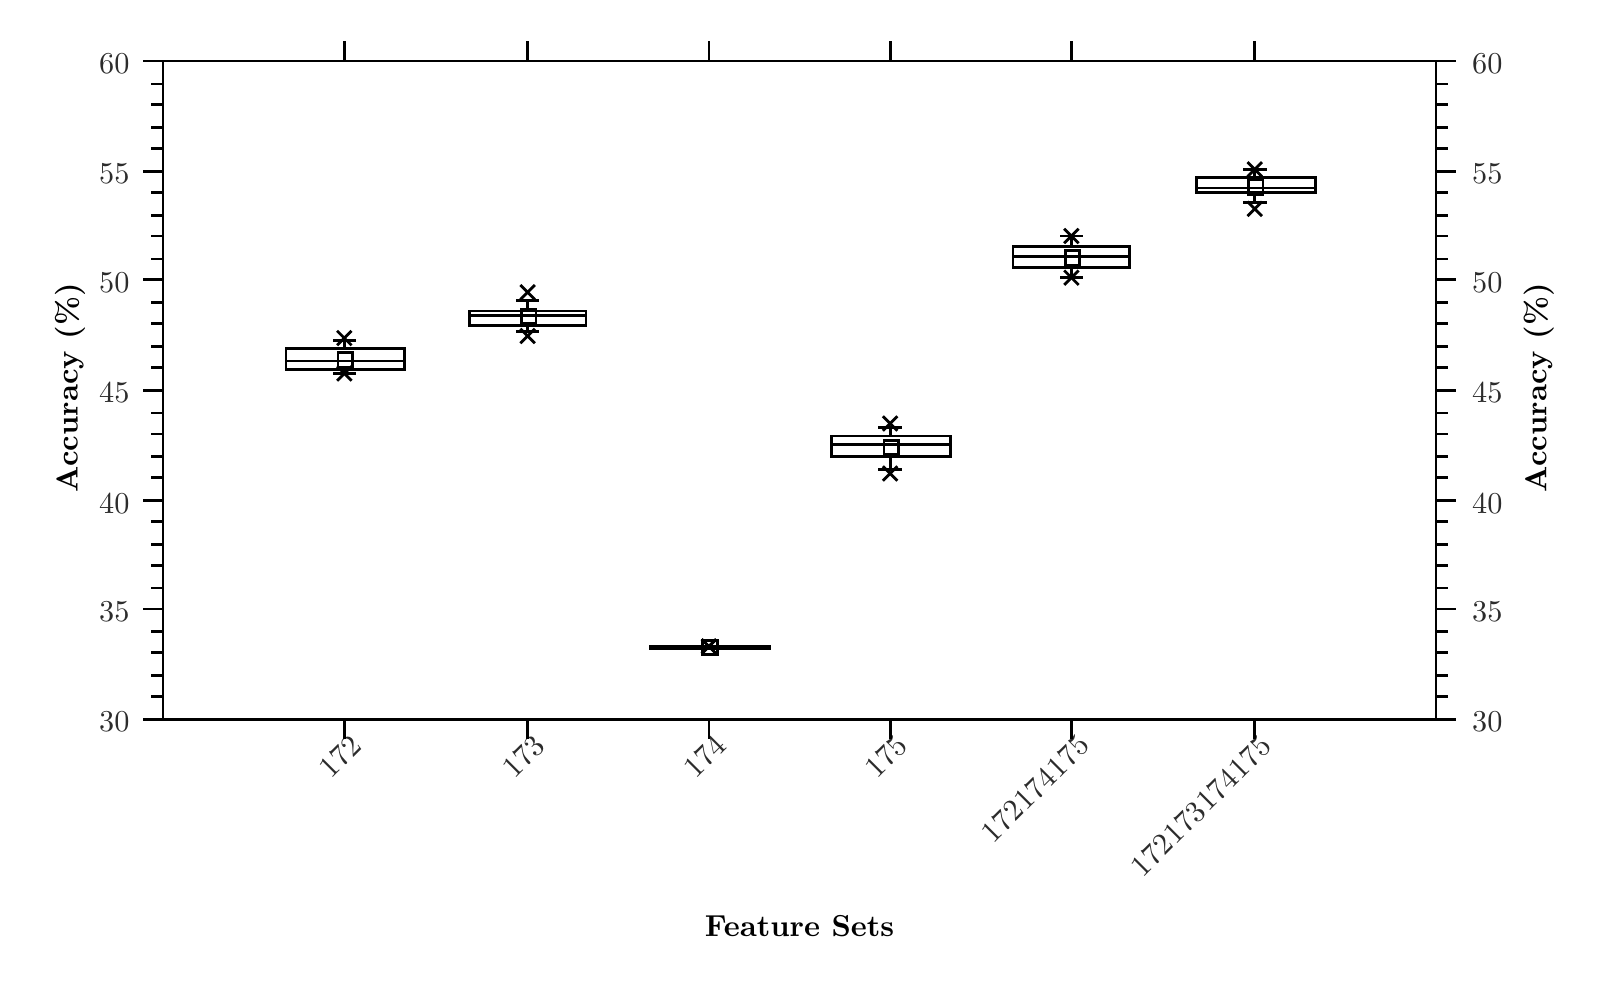
\begin{tikzpicture}{0pt}{0pt}{742pt}{452pt}
	\clip(0pt,452pt) -- (558.587pt,452pt) -- (558.587pt,111.729pt) -- (0pt,111.729pt) -- (0pt,452pt);
\begin{scope}
	\clip(48.9328pt,439.955pt) -- (508.901pt,439.955pt) -- (508.901pt,202.066pt) -- (48.9328pt,202.066pt) -- (48.9328pt,439.955pt);
	\color[rgb]{0,0,0}
	\draw[line width=1pt, line join=miter, line cap=rect](93.3487pt,336.067pt) -- (136.259pt,336.067pt) -- (136.259pt,328.539pt) -- (93.3487pt,328.539pt) -- (93.3487pt,336.067pt);
	\color[rgb]{0,0,0}
	\draw[line width=1pt, line join=miter, line cap=rect](110.663pt,327.033pt) -- (118.192pt,327.033pt);
	\draw[line width=1pt, line join=miter, line cap=rect](110.663pt,339.078pt) -- (118.192pt,339.078pt);
	\draw[line width=1pt, line join=miter, line cap=rect](114.427pt,339.078pt) -- (114.427pt,336.067pt);
	\draw[line width=1pt, line join=miter, line cap=rect](114.427pt,327.033pt) -- (114.427pt,328.539pt);
	\draw[line width=1pt, line join=miter, line cap=rect](93.3487pt,331.55pt) -- (135.506pt,331.55pt);
	\draw[line width=1pt, line join=miter, line cap=rect](112.169pt,329.292pt) -- (116.686pt,324.775pt);
	\draw[line width=1pt, line join=miter, line cap=rect](112.169pt,324.775pt) -- (116.686pt,329.292pt);
	\draw[line width=1pt, line join=miter, line cap=rect](112.169pt,342.089pt) -- (116.686pt,337.572pt);
	\draw[line width=1pt, line join=miter, line cap=rect](112.169pt,337.572pt) -- (116.686pt,342.089pt);
	\draw[line width=1pt, line join=miter, line cap=rect](112.169pt,334.561pt) -- (117.439pt,334.561pt) -- (117.439pt,329.292pt) -- (112.169pt,329.292pt) -- (112.169pt,334.561pt);
	\draw[line width=1pt, line join=miter, line cap=rect](159.596pt,349.618pt) -- (201.754pt,349.618pt) -- (201.754pt,344.348pt) -- (159.596pt,344.348pt) -- (159.596pt,349.618pt);
	\draw[line width=1pt, line join=miter, line cap=rect](176.911pt,342.089pt) -- (184.439pt,342.089pt);
	\draw[line width=1pt, line join=miter, line cap=rect](176.911pt,353.382pt) -- (184.439pt,353.382pt);
	\draw[line width=1pt, line join=miter, line cap=rect](180.675pt,353.382pt) -- (180.675pt,349.618pt);
	\draw[line width=1pt, line join=miter, line cap=rect](180.675pt,342.089pt) -- (180.675pt,344.348pt);
	\draw[line width=1pt, line join=miter, line cap=rect](159.596pt,348.112pt) -- (201.754pt,348.112pt);
	\draw[line width=1pt, line join=miter, line cap=rect](178.417pt,342.842pt) -- (182.933pt,338.325pt);
	\draw[line width=1pt, line join=miter, line cap=rect](178.417pt,338.325pt) -- (182.933pt,342.842pt);
	\draw[line width=1pt, line join=miter, line cap=rect](178.417pt,358.651pt) -- (182.933pt,354.134pt);
	\draw[line width=1pt, line join=miter, line cap=rect](178.417pt,354.134pt) -- (182.933pt,358.651pt);
	\draw[line width=1pt, line join=miter, line cap=rect](178.417pt,350.37pt) -- (183.686pt,350.37pt) -- (183.686pt,345.101pt) -- (178.417pt,345.101pt) -- (178.417pt,350.37pt);
	\draw[line width=1pt, line join=miter, line cap=rect](225.091pt,228.415pt) -- (268.001pt,228.415pt) -- (268.001pt,227.662pt) -- (225.091pt,227.662pt) -- (225.091pt,228.415pt);
	\draw[line width=1pt, line join=miter, line cap=rect](242.406pt,228.415pt) -- (249.934pt,228.415pt);
	\draw[line width=1pt, line join=miter, line cap=rect](242.406pt,228.415pt) -- (249.934pt,228.415pt);
	\draw[line width=1pt, line join=miter, line cap=rect](225.091pt,228.415pt) -- (267.248pt,228.415pt);
	\draw[line width=1pt, line join=miter, line cap=rect](243.911pt,230.673pt) -- (248.428pt,226.156pt);
	\draw[line width=1pt, line join=miter, line cap=rect](243.911pt,226.156pt) -- (248.428pt,230.673pt);
	\draw[line width=1pt, line join=miter, line cap=rect](243.911pt,230.673pt) -- (248.428pt,226.156pt);
	\draw[line width=1pt, line join=miter, line cap=rect](243.911pt,226.156pt) -- (248.428pt,230.673pt);
	\draw[line width=1pt, line join=miter, line cap=rect](243.911pt,230.673pt) -- (249.181pt,230.673pt) -- (249.181pt,225.403pt) -- (243.911pt,225.403pt) -- (243.911pt,230.673pt);
	\draw[line width=1pt, line join=miter, line cap=rect](290.586pt,304.449pt) -- (333.496pt,304.449pt) -- (333.496pt,296.921pt) -- (290.586pt,296.921pt) -- (290.586pt,304.449pt);
	\draw[line width=1pt, line join=miter, line cap=rect](307.9pt,292.404pt) -- (315.428pt,292.404pt);
	\draw[line width=1pt, line join=miter, line cap=rect](307.9pt,307.46pt) -- (315.428pt,307.46pt);
	\draw[line width=1pt, line join=miter, line cap=rect](311.664pt,307.46pt) -- (311.664pt,304.449pt);
	\draw[line width=1pt, line join=miter, line cap=rect](311.664pt,292.404pt) -- (311.664pt,296.921pt);
	\draw[line width=1pt, line join=miter, line cap=rect](290.586pt,301.438pt) -- (332.743pt,301.438pt);
	\draw[line width=1pt, line join=miter, line cap=rect](309.406pt,293.157pt) -- (313.923pt,288.64pt);
	\draw[line width=1pt, line join=miter, line cap=rect](309.406pt,288.64pt) -- (313.923pt,293.157pt);
	\draw[line width=1pt, line join=miter, line cap=rect](309.406pt,311.224pt) -- (313.923pt,306.707pt);
	\draw[line width=1pt, line join=miter, line cap=rect](309.406pt,306.707pt) -- (313.923pt,311.224pt);
	\draw[line width=1pt, line join=miter, line cap=rect](309.406pt,302.943pt) -- (314.676pt,302.943pt) -- (314.676pt,297.673pt) -- (309.406pt,297.673pt) -- (309.406pt,302.943pt);
	\draw[line width=1pt, line join=miter, line cap=rect](356.08pt,372.955pt) -- (398.238pt,372.955pt) -- (398.238pt,365.427pt) -- (356.08pt,365.427pt) -- (356.08pt,372.955pt);
	\draw[line width=1pt, line join=miter, line cap=rect](373.395pt,361.663pt) -- (380.923pt,361.663pt);
	\draw[line width=1pt, line join=miter, line cap=rect](373.395pt,376.719pt) -- (380.923pt,376.719pt);
	\draw[line width=1pt, line join=miter, line cap=rect](377.159pt,376.719pt) -- (377.159pt,372.955pt);
	\draw[line width=1pt, line join=miter, line cap=rect](377.159pt,361.663pt) -- (377.159pt,365.427pt);
	\draw[line width=1pt, line join=miter, line cap=rect](356.08pt,369.191pt) -- (398.238pt,369.191pt);
	\draw[line width=1pt, line join=miter, line cap=rect](374.901pt,363.921pt) -- (379.418pt,359.404pt);
	\draw[line width=1pt, line join=miter, line cap=rect](374.901pt,359.404pt) -- (379.418pt,363.921pt);
	\draw[line width=1pt, line join=miter, line cap=rect](374.901pt,378.977pt) -- (379.418pt,374.46pt);
	\draw[line width=1pt, line join=miter, line cap=rect](374.901pt,374.46pt) -- (379.418pt,378.977pt);
	\draw[line width=1pt, line join=miter, line cap=rect](374.901pt,371.449pt) -- (380.17pt,371.449pt) -- (380.17pt,366.179pt) -- (374.901pt,366.179pt) -- (374.901pt,371.449pt);
	\draw[line width=1pt, line join=miter, line cap=rect](422.328pt,397.798pt) -- (465.238pt,397.798pt) -- (465.238pt,392.528pt) -- (422.328pt,392.528pt) -- (422.328pt,397.798pt);
	\draw[line width=1pt, line join=miter, line cap=rect](439.642pt,388.764pt) -- (447.171pt,388.764pt);
	\draw[line width=1pt, line join=miter, line cap=rect](439.642pt,400.809pt) -- (447.171pt,400.809pt);
	\draw[line width=1pt, line join=miter, line cap=rect](443.407pt,400.809pt) -- (443.407pt,397.798pt);
	\draw[line width=1pt, line join=miter, line cap=rect](443.407pt,388.764pt) -- (443.407pt,392.528pt);
	\draw[line width=1pt, line join=miter, line cap=rect](422.328pt,394.033pt) -- (464.485pt,394.033pt);
	\draw[line width=1pt, line join=miter, line cap=rect](441.148pt,388.764pt) -- (445.665pt,384.247pt);
	\draw[line width=1pt, line join=miter, line cap=rect](441.148pt,384.247pt) -- (445.665pt,388.764pt);
	\draw[line width=1pt, line join=miter, line cap=rect](441.148pt,403.067pt) -- (445.665pt,398.55pt);
	\draw[line width=1pt, line join=miter, line cap=rect](441.148pt,398.55pt) -- (445.665pt,403.067pt);
	\draw[line width=1pt, line join=miter, line cap=rect](441.148pt,397.045pt) -- (446.418pt,397.045pt) -- (446.418pt,391.775pt) -- (441.148pt,391.775pt) -- (441.148pt,397.045pt);
\end{scope}
\begin{scope}
	\color[rgb]{0,0,0}
	\pgftext[center, base, at={\pgfpoint{18.0675pt}{321.763pt}},rotate=90]{\fontsize{11}{0}\selectfont{\textbf{Accuracy (\%)}}}
	\color[rgb]{0.172549,0.172549,0.172549}
	\pgftext[center, base, at={\pgfpoint{31.3358pt}{197.549pt}}]{\fontsize{11}{0}\selectfont{30}}
	\pgftext[center, base, at={\pgfpoint{31.3358pt}{237.448pt}}]{\fontsize{11}{0}\selectfont{35}}
	\pgftext[center, base, at={\pgfpoint{31.3358pt}{276.595pt}}]{\fontsize{11}{0}\selectfont{40}}
	\pgftext[center, base, at={\pgfpoint{31.3358pt}{316.494pt}}]{\fontsize{11}{0}\selectfont{45}}
	\pgftext[center, base, at={\pgfpoint{31.3358pt}{356.393pt}}]{\fontsize{11}{0}\selectfont{50}}
	\pgftext[center, base, at={\pgfpoint{31.3358pt}{395.539pt}}]{\fontsize{11}{0}\selectfont{55}}
	\pgftext[center, base, at={\pgfpoint{31.3358pt}{435.438pt}}]{\fontsize{11}{0}\selectfont{60}}
	\color[rgb]{0,0,0}
	\draw[line width=1pt, line join=bevel, line cap=rect](48.9328pt,210.347pt) -- (45.1688pt,210.347pt);
	\draw[line width=1pt, line join=bevel, line cap=rect](48.9328pt,217.875pt) -- (45.1688pt,217.875pt);
	\draw[line width=1pt, line join=bevel, line cap=rect](48.9328pt,226.156pt) -- (45.1688pt,226.156pt);
	\draw[line width=1pt, line join=bevel, line cap=rect](48.9328pt,233.684pt) -- (45.1688pt,233.684pt);
	\draw[line width=1pt, line join=bevel, line cap=rect](48.9328pt,249.493pt) -- (45.1688pt,249.493pt);
	\draw[line width=1pt, line join=bevel, line cap=rect](48.9328pt,257.774pt) -- (45.1688pt,257.774pt);
	\draw[line width=1pt, line join=bevel, line cap=rect](48.9328pt,265.303pt) -- (45.1688pt,265.303pt);
	\draw[line width=1pt, line join=bevel, line cap=rect](48.9328pt,273.583pt) -- (45.1688pt,273.583pt);
	\draw[line width=1pt, line join=bevel, line cap=rect](48.9328pt,289.393pt) -- (45.1688pt,289.393pt);
	\draw[line width=1pt, line join=bevel, line cap=rect](48.9328pt,296.921pt) -- (45.1688pt,296.921pt);
	\draw[line width=1pt, line join=bevel, line cap=rect](48.9328pt,305.202pt) -- (45.1688pt,305.202pt);
	\draw[line width=1pt, line join=bevel, line cap=rect](48.9328pt,312.73pt) -- (45.1688pt,312.73pt);
	\draw[line width=1pt, line join=bevel, line cap=rect](48.9328pt,329.292pt) -- (45.1688pt,329.292pt);
	\draw[line width=1pt, line join=bevel, line cap=rect](48.9328pt,336.82pt) -- (45.1688pt,336.82pt);
	\draw[line width=1pt, line join=bevel, line cap=rect](48.9328pt,345.101pt) -- (45.1688pt,345.101pt);
	\draw[line width=1pt, line join=bevel, line cap=rect](48.9328pt,352.629pt) -- (45.1688pt,352.629pt);
	\draw[line width=1pt, line join=bevel, line cap=rect](48.9328pt,368.438pt) -- (45.1688pt,368.438pt);
	\draw[line width=1pt, line join=bevel, line cap=rect](48.9328pt,376.719pt) -- (45.1688pt,376.719pt);
	\draw[line width=1pt, line join=bevel, line cap=rect](48.9328pt,384.247pt) -- (45.1688pt,384.247pt);
	\draw[line width=1pt, line join=bevel, line cap=rect](48.9328pt,392.528pt) -- (45.1688pt,392.528pt);
	\draw[line width=1pt, line join=bevel, line cap=rect](48.9328pt,408.337pt) -- (45.1688pt,408.337pt);
	\draw[line width=1pt, line join=bevel, line cap=rect](48.9328pt,415.865pt) -- (45.1688pt,415.865pt);
	\draw[line width=1pt, line join=bevel, line cap=rect](48.9328pt,424.146pt) -- (45.1688pt,424.146pt);
	\draw[line width=1pt, line join=bevel, line cap=rect](48.9328pt,431.674pt) -- (45.1688pt,431.674pt);
	\draw[line width=1pt, line join=bevel, line cap=rect](48.9328pt,202.066pt) -- (42.1575pt,202.066pt);
	\draw[line width=1pt, line join=bevel, line cap=rect](48.9328pt,241.965pt) -- (42.1575pt,241.965pt);
	\draw[line width=1pt, line join=bevel, line cap=rect](48.9328pt,281.112pt) -- (42.1575pt,281.112pt);
	\draw[line width=1pt, line join=bevel, line cap=rect](48.9328pt,321.011pt) -- (42.1575pt,321.011pt);
	\draw[line width=1pt, line join=bevel, line cap=rect](48.9328pt,360.91pt) -- (42.1575pt,360.91pt);
	\draw[line width=1pt, line join=bevel, line cap=rect](48.9328pt,400.056pt) -- (42.1575pt,400.056pt);
	\draw[line width=1pt, line join=bevel, line cap=rect](48.9328pt,439.955pt) -- (42.1575pt,439.955pt);
	\draw[line width=1pt, line join=bevel, line cap=rect](48.9328pt,439.955pt) -- (48.9328pt,202.066pt);
	\pgftext[center, base, at={\pgfpoint{548.8pt}{321.763pt}},rotate=90]{\fontsize{11}{0}\selectfont{\textbf{Accuracy (\%)}}}
	\color[rgb]{0.172549,0.172549,0.172549}
	\pgftext[center, base, at={\pgfpoint{527.439pt}{197.549pt}}]{\fontsize{11}{0}\selectfont{30}}
	\pgftext[center, base, at={\pgfpoint{527.439pt}{237.448pt}}]{\fontsize{11}{0}\selectfont{35}}
	\pgftext[center, base, at={\pgfpoint{527.439pt}{276.595pt}}]{\fontsize{11}{0}\selectfont{40}}
	\pgftext[center, base, at={\pgfpoint{527.439pt}{316.494pt}}]{\fontsize{11}{0}\selectfont{45}}
	\pgftext[center, base, at={\pgfpoint{527.439pt}{356.393pt}}]{\fontsize{11}{0}\selectfont{50}}
	\pgftext[center, base, at={\pgfpoint{527.439pt}{395.539pt}}]{\fontsize{11}{0}\selectfont{55}}
	\pgftext[center, base, at={\pgfpoint{527.439pt}{435.438pt}}]{\fontsize{11}{0}\selectfont{60}}
	\color[rgb]{0,0,0}
	\draw[line width=1pt, line join=bevel, line cap=rect](508.901pt,210.347pt) -- (512.665pt,210.347pt);
	\draw[line width=1pt, line join=bevel, line cap=rect](508.901pt,217.875pt) -- (512.665pt,217.875pt);
	\draw[line width=1pt, line join=bevel, line cap=rect](508.901pt,226.156pt) -- (512.665pt,226.156pt);
	\draw[line width=1pt, line join=bevel, line cap=rect](508.901pt,233.684pt) -- (512.665pt,233.684pt);
	\draw[line width=1pt, line join=bevel, line cap=rect](508.901pt,249.493pt) -- (512.665pt,249.493pt);
	\draw[line width=1pt, line join=bevel, line cap=rect](508.901pt,257.774pt) -- (512.665pt,257.774pt);
	\draw[line width=1pt, line join=bevel, line cap=rect](508.901pt,265.303pt) -- (512.665pt,265.303pt);
	\draw[line width=1pt, line join=bevel, line cap=rect](508.901pt,273.583pt) -- (512.665pt,273.583pt);
	\draw[line width=1pt, line join=bevel, line cap=rect](508.901pt,289.393pt) -- (512.665pt,289.393pt);
	\draw[line width=1pt, line join=bevel, line cap=rect](508.901pt,296.921pt) -- (512.665pt,296.921pt);
	\draw[line width=1pt, line join=bevel, line cap=rect](508.901pt,305.202pt) -- (512.665pt,305.202pt);
	\draw[line width=1pt, line join=bevel, line cap=rect](508.901pt,312.73pt) -- (512.665pt,312.73pt);
	\draw[line width=1pt, line join=bevel, line cap=rect](508.901pt,329.292pt) -- (512.665pt,329.292pt);
	\draw[line width=1pt, line join=bevel, line cap=rect](508.901pt,336.82pt) -- (512.665pt,336.82pt);
	\draw[line width=1pt, line join=bevel, line cap=rect](508.901pt,345.101pt) -- (512.665pt,345.101pt);
	\draw[line width=1pt, line join=bevel, line cap=rect](508.901pt,352.629pt) -- (512.665pt,352.629pt);
	\draw[line width=1pt, line join=bevel, line cap=rect](508.901pt,368.438pt) -- (512.665pt,368.438pt);
	\draw[line width=1pt, line join=bevel, line cap=rect](508.901pt,376.719pt) -- (512.665pt,376.719pt);
	\draw[line width=1pt, line join=bevel, line cap=rect](508.901pt,384.247pt) -- (512.665pt,384.247pt);
	\draw[line width=1pt, line join=bevel, line cap=rect](508.901pt,392.528pt) -- (512.665pt,392.528pt);
	\draw[line width=1pt, line join=bevel, line cap=rect](508.901pt,408.337pt) -- (512.665pt,408.337pt);
	\draw[line width=1pt, line join=bevel, line cap=rect](508.901pt,415.865pt) -- (512.665pt,415.865pt);
	\draw[line width=1pt, line join=bevel, line cap=rect](508.901pt,424.146pt) -- (512.665pt,424.146pt);
	\draw[line width=1pt, line join=bevel, line cap=rect](508.901pt,431.674pt) -- (512.665pt,431.674pt);
	\draw[line width=1pt, line join=bevel, line cap=rect](508.901pt,202.066pt) -- (515.677pt,202.066pt);
	\draw[line width=1pt, line join=bevel, line cap=rect](508.901pt,241.965pt) -- (515.677pt,241.965pt);
	\draw[line width=1pt, line join=bevel, line cap=rect](508.901pt,281.112pt) -- (515.677pt,281.112pt);
	\draw[line width=1pt, line join=bevel, line cap=rect](508.901pt,321.011pt) -- (515.677pt,321.011pt);
	\draw[line width=1pt, line join=bevel, line cap=rect](508.901pt,360.91pt) -- (515.677pt,360.91pt);
	\draw[line width=1pt, line join=bevel, line cap=rect](508.901pt,400.056pt) -- (515.677pt,400.056pt);
	\draw[line width=1pt, line join=bevel, line cap=rect](508.901pt,439.955pt) -- (515.677pt,439.955pt);
	\draw[line width=1pt, line join=bevel, line cap=rect](508.901pt,439.955pt) -- (508.901pt,202.066pt);
	\pgftext[center, base, at={\pgfpoint{278.911pt}{123.774pt}}]{\fontsize{11}{0}\selectfont{\textbf{Feature Sets}}}
	\color[rgb]{0.172549,0.172549,0.172549}
	\pgftext[center, base, at={\pgfpoint{115.392pt}{186.104pt}},rotate=45]{\fontsize{11}{0}\selectfont{\ding{172}}}
	\pgftext[center, base, at={\pgfpoint{181.64pt}{186.104pt}},rotate=45]{\fontsize{11}{0}\selectfont{\ding{173}}}
	\pgftext[center, base, at={\pgfpoint{247.135pt}{186.104pt}},rotate=45]{\fontsize{11}{0}\selectfont{\ding{174}}}
	\pgftext[center, base, at={\pgfpoint{312.629pt}{186.104pt}},rotate=45]{\fontsize{11}{0}\selectfont{\ding{175}}}
	\pgftext[center, base, at={\pgfpoint{354.702pt}{162.682pt}},rotate=45]{\fontsize{11}{0}\selectfont{\ding{172}}}
	\pgftext[center, base, at={\pgfpoint{366.513pt}{174.493pt}},rotate=45]{\fontsize{11}{0}\selectfont{\ding{174}}}
	\pgftext[center, base, at={\pgfpoint{378.324pt}{186.303pt}},rotate=45]{\fontsize{11}{0}\selectfont{\ding{175}}}
	\pgftext[center, base, at={\pgfpoint{408.706pt}{150.439pt}},rotate=45]{\fontsize{11}{0}\selectfont{\ding{172}}}
	\pgftext[center, base, at={\pgfpoint{420.517pt}{162.249pt}},rotate=45]{\fontsize{11}{0}\selectfont{\ding{173}}}
	\pgftext[center, base, at={\pgfpoint{432.328pt}{174.06pt}},rotate=45]{\fontsize{11}{0}\selectfont{\ding{174}}}
	\pgftext[center, base, at={\pgfpoint{444.139pt}{185.871pt}},rotate=45]{\fontsize{11}{0}\selectfont{\ding{175}}}
	\color[rgb]{0,0,0}
	\draw[line width=1pt, line join=bevel, line cap=rect](114.427pt,202.066pt) -- (114.427pt,195.291pt);
	\draw[line width=1pt, line join=bevel, line cap=rect](180.675pt,202.066pt) -- (180.675pt,195.291pt);
	\draw[line width=1pt, line join=bevel, line cap=rect](246.17pt,202.066pt) -- (246.17pt,195.291pt);
	\draw[line width=1pt, line join=bevel, line cap=rect](311.664pt,202.066pt) -- (311.664pt,195.291pt);
	\draw[line width=1pt, line join=bevel, line cap=rect](377.159pt,202.066pt) -- (377.159pt,195.291pt);
	\draw[line width=1pt, line join=bevel, line cap=rect](443.407pt,202.066pt) -- (443.407pt,195.291pt);
	\draw[line width=1pt, line join=bevel, line cap=rect](48.9328pt,202.066pt) -- (508.901pt,202.066pt);
	\draw[line width=1pt, line join=bevel, line cap=rect](114.427pt,439.955pt) -- (114.427pt,446.73pt);
	\draw[line width=1pt, line join=bevel, line cap=rect](180.675pt,439.955pt) -- (180.675pt,446.73pt);
	\draw[line width=1pt, line join=bevel, line cap=rect](246.17pt,439.955pt) -- (246.17pt,446.73pt);
	\draw[line width=1pt, line join=bevel, line cap=rect](311.664pt,439.955pt) -- (311.664pt,446.73pt);
	\draw[line width=1pt, line join=bevel, line cap=rect](377.159pt,439.955pt) -- (377.159pt,446.73pt);
	\draw[line width=1pt, line join=bevel, line cap=rect](443.407pt,439.955pt) -- (443.407pt,446.73pt);
	\draw[line width=1pt, line join=bevel, line cap=rect](48.9328pt,439.955pt) -- (508.901pt,439.955pt);
\end{scope}
\end{tikzpicture}

  \end{adjustbox}
  \caption{Method-level cross-validation accuracy of feature sets on the \emph{all} subject.}
  \vspace{2mm}
  \hrule
  \label{fig:all_cross_validation_features_method_graph}
\end{figure}

We use the LIBSVM~\cite{CL11} library to perform the 10-fold cross-validation. To evaluate the cross-validation accuracy of the acquired data we randomly under-sample the data to balance the amount of instances within each category. We utilize 191 instances of class-level and 1104 instances of method-level source code units from each category, these values are chosen to maximize the number of instances of the minority category using random under-sampling.

In Figure~\ref{fig:all_cross_validation_features_class_graph}~\&~\ref{fig:all_cross_validation_features_method_graph} we present the cross-validation accuracy of class- and method-level source code units on the \emph{all} subject over 10 executions to account for the random undersampling of our data. In addition we evaluate the cross-validation of each individual set of features to understand their individual impacts on cross-validation accuracy. The baseline to outperform is random in terms of cross-validation accuracy, in our case since we undersample our three categories random accuracy is 33.33\%. We can see that all feature sets are able to outperform random which indicates that there is some predictive power in the selected feature sets\footnote{Feature set \ding{174} for method-level source code units (Figure~\ref{fig:all_cross_validation_features_method_graph}) does not add any value (as it is specifically tailor for class-level source code units), and thus performs as random}. We include a subset of all features (feature sets \ding{172} \ding{174} \ding{175}) to show the effects of merging only the source and test metrics (excluding coverage feature set \ding{173}). We can clearly see that by using all feature sets together we can acquire higher cross-validation accuracy then using the feature sets alone. There is a greater difference in the cross-validation accuracy of all feature sets in the method-level source code units, which is fine as method-level source code predictions are finer-grain. This supports our intuition using various metrics together we can predict the mutation scores of source code units well.


\subsection{Feature Selection}
\label{subsec:experiment_feature_selection}
In machine learning typically one gathers as many features as possible to supply enough data such that the learning algorithms can make accurate predictions. The problem at hand (i.e., being able to predict the correct category of a vector) is that some features will be redundant, irrelevant or detrimental to the predictive efforts. With proper features the prediction performance can improve, or remain closely the same with less information required. With a lessen feature load the actual performance (i.e., with respect to computational resources required) will improve. By using \emph{feature selection} it is possible to utilize a subset of the features that hopefully improve/retain the predictive performance with less required data~\cite{GE03,BL97}.

There are several approaches to dealing with feature selection, in particular \emph{filter} and \emph{wrapper}. Filters assess the quality/merits of features solely from the data alone as a preprocessing step~\cite{JKP94,BL97}. Various algorithms and measures can be used as a filter (i.e., information gain~\cite{GE03}, correlation~\cite{Hal99}, FOCUS~\cite{AD91}, Relief~\cite{KR92}, etc\ldots). An alternative to filters are wrappers, which evaluates the actual performance of features using the classifier. Wrappers treat the classifier as a black-box and assess the performance using various subsets of features by using the actual predictor~\cite{JKP94,BL97}. Wrappers provide a more accurate and effective means in finding appropriate features, though inefficient as the classification process must occur many times using cross-validation with different features~\cite{KJ97}.

Given that we have over 3000 vectors (with undersampling in effect) with 15 features for the method-level dataset a wrapper approach can be very costly. A wrapper approach might prove more effective as found by Kohavi and John~\cite{KJ97}. For our research we decided against a wrapper approach due to the high computational cost involved. As an alternative to a wrapper approach we use Hall's \gls{cfs} filter which is based on the follow definition: \emph{``A good feature subset is one that contains features highly correlated with (predictive of) the class, yet uncorrelated with (not predictive of) each other''}~\cite{Hal99}. To do this we utilize the \gls{cfs} implementation found in the machine learning toolkit Weka~\cite{HFH+09}.

We undersampled ten times the available data of the combination of our 8 subjects (\emph{all}) for both class- and method-level. Using the 10 different undersampled set of vectors that contain all our features we then apply the \gls{cfs} filter to each which produce an ascending order of features with respect to their correlation ranking (i.e., how effective the feature is with respect to others). To account for the undersampling we apply the \gls{cfs} filter on each of the 10 undersampled sets of data. We then use a simple rank summation to tally the results (i.e., ascending rank \emph{n} has a value of \emph{n}), which then allows us to have a overall ranking of the features across the 10 different undersampled data sets. We then can remove the least useful feature one-at-a-time and observe the new 10-fold cross-validation performance of the classifier using a subset of all the features. The results are presented in Figure~\ref{?}.


\subsection{Prediction}
\label{subsec:experiment_prediction}
By using LIBSVM we want to train a classifier such that it can predict well on \emph{unknown data}. Parameter selection and the training/testing data sets play an important role in making a good classifier. Ultimately, we want to obtain a classifier that is able to \emph{generalize} to new unknown data. In our specific case since we have 8 different subjects (that are most likely not similar to each other in terms of features) in which we want to maximize our generalizability. We used cross-validation in Section~\ref{subsec:experiment_cross_validation} as it mitigates the overfitting problem introduced by training (i.e., a model becomes specifically tuned for the training data set)~\cite{HCL03}. Parameter selection also occurred automatically using a grid search approach to find a set of parameters that maximized the cross-validation accuracy on the training data set. We were able to achieve a cross-validation accuracy of 0.542662 using all features which performs much better then a random approach (i.e., around 0.333333), though does this generalize to unknown data?

To explore this generalization problem we conducted a number of tests where we use LIBSVM's \emph{easy script} to find the best parameters that maximize cross-validation accuracy and then apply the classifier to unknown data. As we are still using undersampling we conduct each experiment 10 times to determine the mean and standard deviation in prediction accuracy. We consider the prediction accuracy on the remaining unknown data (i.e., what is left from the undersampling) of the experimental subject being used (see Table~\ref{?}). We also looked at the prediction accuracy on completely unknown subject by training on the other 7 \emph{all\_but\_<subject>} sets and predicting on the unknown subject (see Table~\ref{?}).


\subsection{Optimization \& Generalization}
\label{subsec:experiment_optimization_generalization}
We keep track of the frequency of parameter pairs selected over all the prediction experiments conducted in Section~\ref{subsec:experiment_prediction}. As shown in Table~\ref{?} we can see that a large number of parameter pairings are used to maximize the cross-validation accuracy of the training data sets, before using them for prediction. This indicates that the classifiers are being tuned specifically to maximize the cross-validation accuracy, and due to undersampling different parameters are being used to ensure this maximization. To encourage generalization of unknown projects and data we ideally want to find a parameter pairing that maximizes generalizability and classification performance.

We noticed that in some situations accuracy is not the best measure for a classifier's effectiveness. For example, consider the following situation: Given imbalanced data for the testing/unknown data set the accuracy could misrepresent the performance of the classifier. If we look at Figure~\ref{fig:raw_output_bad}~\&~\ref{fig:raw_output_good} we can see the raw outputs of our classifier using two different sets of parameters. We can see a confusion matrix for both a good classifier and bad classifier. We can see in Figure~\ref{fig:raw_output_bad} that the majority of predictions fall in category \texttt{2}, with very few in category \texttt{0}, and none in the remaining category. This data set does constitute imbalanced data as around 56\% of the data belongs to category \texttt{2}. We can see that even with the biased predictions made towards the majority category the accuracy of the prediction is 0.561680. In contrast to the the raw output presented in Figure~\ref{fig:raw_output_good} we can see that the accuracy is slightly lower at 0.543307. Now even though the accuracy in the second example is slightly lower we can consider it a superior classifier to the former as it actually treats the three categories in a more unbiased fashion (i.e., one category is not receiving the majority of predictions like the previous example). To alleviate this problem we consider other measurements that can be used to assess the predictive capabilities of classifiers, in particular we consider the following measure:

\begin{itemize}
  \item \textbf{F-score} represents the harmonic mean of the recall and precision for a category.~\cite{SJS06}
  \begin{equation}
    \emph{$\text{F-score} = 2*\frac{recall * precision}{recall + precision}$}
    \label{equ:f_score}
  \end{equation}

  \item \textbf{Balanced Accuracy} represents the average accuracy obtained on the category.~\cite{BOSB10, SJS06}
  \begin{equation}
    \emph{$\text{balanced accuracy} = \frac{recall + specificity}{2}$}
    \label{equ:balanced_area_under_curve}
  \end{equation}

  \item \textbf{Youden's Index} represents the classifier's ability to avoid failure. It can also be calculated using the balanced accuracy.~\cite{SJS06}
  \begin{equation}
    \emph{$\text{youden's index} = recall - ( 1 - specificity)$}
    \label{equ:youden_index_a}
  \end{equation}
  \begin{equation}
    \emph{$\text{youden's index} = 2 * \text{balanced accuracy} - 1$}
    \label{equ:youden_index_b}
  \end{equation}
\end{itemize}

\begin{landscape}
  \begin{figure}
    \centering
    \begin{minipage}{22.0cm}
    \scriptsize{
    \lstinputlisting[language=Java, basicstyle=\footnotesize\ttfamily,]{listings/raw_output_bad.txt}
    }
    \end{minipage}
    \caption{Raw output of running \texttt{all\_but\_jsoup} (training on all but \texttt{jsoup} then predicting on it) using the parameters \emph{cost}=1 and \emph{gamma}=0.001.}
    \vspace{2mm}
    \hrule
    \label{fig:raw_output_bad}
  \end{figure}

  \begin{figure}
    \centering
    \begin{minipage}{22.0cm}
    \scriptsize{
    \lstinputlisting[language=Java, basicstyle=\footnotesize\ttfamily,]{listings/raw_output_good.txt}
    }
    \end{minipage}
    \caption{Raw output of running \texttt{all\_but\_jsoup} (training on all but \texttt{jsoup} then predicting on it) using the parameters \emph{cost}=10 and \emph{gamma}=10.}
    \vspace{2mm}
    \hrule
    \label{fig:raw_output_good}
  \end{figure}
\end{landscape}


\section{Summary}
\label{sec:experiment_summary}
In this chapter we covered the following topics that are considered background material for the approach presented in this thesis:

\begin{itemize}
  \item In Section~\ref{sec:experiment_setup} we covered how our experimental setup with respect to machine setup and the different types of evaluations we will perform.
  \item In Section~\ref{sec:experiment_subjects} we covered the 8 experimental subjects what machine learning and how it can be for supervised and unsupervised classification technique. We specifically cover how \gls{svm}s work.
  \item In Section~\ref{sec:experiment_results} we covered metrics, specifically source code and test suite metrics. We explain how source code metrics can be used to identify \emph{code smells} and some examples of these metrics. We also introduce several approaches to test suite metrics using a combination of source code metrics on JUnit test cases as well as coverage metrics.
\end{itemize}
